\chapter{Vorgehen}
- was für frameworks wurden verwendet (vs code, react, xstate, chakra ui)

episodes identification and association (EIA) enables the interface to recognize user action plans by tracing
and analyzing a user’s action sequences. Implementing this approach involves five important issues:
\begin{itemize}
    \item \textbf{Observing the interaction between a user and a software application}. We might lose data 
    because of limitations in the types of events we can perceive. So, to extract as much useful
    information about a user’s intentions and needs as possible, we must identify various low-level
    interface events from available data.
    \item \textbf{Identifying different episodes from the actions we observe in user–computer interaction}. We
    must formulate several important classes from user interface data—for example, keyboard
    typing, menu selection, and button clicking. We consider each action a basic episode. These
    observable clues will help us recognize a user’s intention.
    \item \textbf{Recognizing user behavior patterns}. To reveal hidden patterns in the streams of events we
    retrieve, we need a language or algorithms for representing and computing the events into
    associated patterns. Moreover, the AUI should be able to compose new events from previously
    modeled events and build or modify the transformation functions for the modeled events.
    \item \textbf{Adaptively helping users according to recognized user plans}. When the interface recognizes
    that the user is about to execute a certain plan, it should offer assistance. The user can configure
    the interface with his or her preferences on where and how to display the proposed help.
    \item \textbf{Building user profiles that will enable personalized interactions}. Profiles store both userdefined
    preference information and systemdetected user behavior patterns. The system updates a profile whenever it detects a change
    in user behavior patterns.
\end{itemize}

\begin{figure}[h]
    \centering
    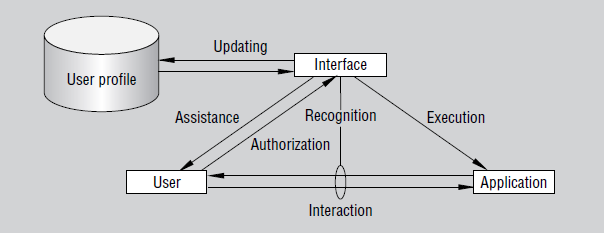
\includegraphics[height=.385\textwidth]{Shematic-AUI.png}
    \caption{Schematic of an adaptive User Interface}
\end{figure}
\newpage
The interface tracks interaction between a user and an application software system and tries to identify consistent user behavior patterns.
On the basis of these patterns, it can interact with the software on the user’s behalf whenever the user authorizes the interface to do
so. The interface might take a while to detect user patterns if it starts from scratch every time the user uses the software. Alternatively,
the AUI can build a user profile that includes all the patterns recognized in past interaction sessions. As it detects new patterns, it updates
the profile.

\chapter{Umsetzung}

